\documentclass[11pt, aspectratio=43]{beamer}
\usetheme[blue]{cbflec}% loading the custom theme

% Auxillary packages that you may use; not necessary for the custom theme
\usepackage{charter}
\usepackage{threeparttable}
\usepackage{booktabs}
\usepackage{hyperref}
\hypersetup{colorlinks=true,
urlcolor=purple, 
}

\title{A Simple Beamer Theme for Lectures}
\subtitle{theme \textbf{cbflec} for colorblind-friendly slides}
%\author{Name Surname \\ \texttt{email@adress.edu}}
\date{\today}
%\institute{Your University}


\begin{document}
\section{\inserttitle}
\begin{frame}[plain] % plain frame to suppress the page number on the title page
    \titlepage
\end{frame}

\subsection{Colors}
\begin{tframe}
    \Large Why different colors?
\end{tframe}

\begin{frame}{Color Picks}
    \begin{itemize}
        \item Colors suitable for color-blind readers based on \href{https://www.nature.com/articles/nmeth.1618}{Wong (2011)}
    \end{itemize}
    \vspace{1ex}
    \begin{minipage}{\textwidth}
        \centering
        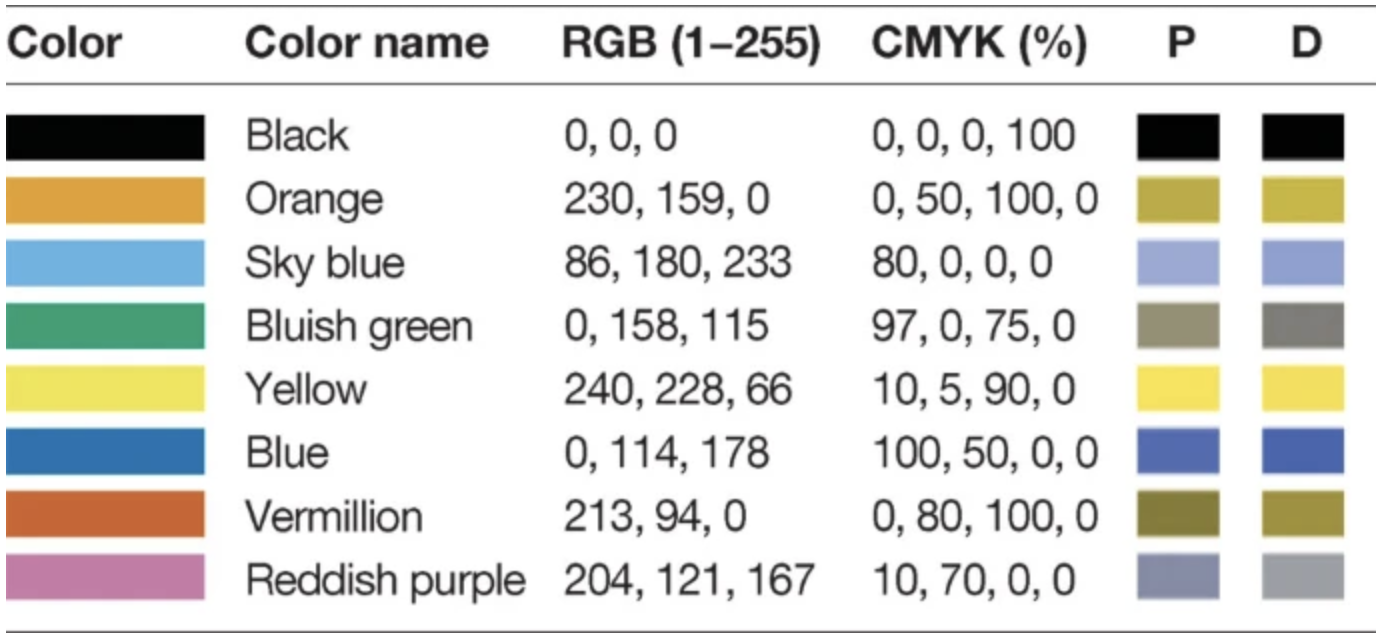
\includegraphics[scale=0.4]{cbf_colors.png}\\
        \footnotesize Source: Wong (2011)
    \end{minipage}
\end{frame}

\begin{frame}{Color Picks, Cont.}
    \begin{itemize}
        \item \textcolor{blue}{Blue} for
        \begin{itemize}
            \item title page
            \item frame title (bold series)
            \item itemize/enumerate item markers
            \item transition frame
        \end{itemize}
        \item \textcolor{red}{Red} for
        \begin{itemize}
            \item highlighting 
            \item description item
            \item alert environment
        \end{itemize}
        \item \textcolor{yellow}{Yellow} as an alternative color for the transition frame background 
        \item \textcolor{orange}{Orange} for the block environment
        \item \textcolor{teal}{Teal} for the example environment
    \end{itemize}
\end{frame}

\begin{frame}[fragile]
    \frametitle{Title Page}
    \begin{itemize}
        \item Title page is inspired by \href{https://blog.hamaluik.ca/posts/better-beamer-themes/}{Kenton Hamaluik}
        \item I don't like to have author and institution information on lecture slides
        \item My students know these already!
        \item Yet \textbf{cbflec} allows you to have them on the title page. Try!
        \item It also works fine with aspect ratio 16:9, which I prefer for my lectures (\verb!\documentclass[aspectratio=169]{beamer}!)
    \end{itemize}
\end{frame}

\begin{frame}{Descriptions}
    \begin{itemize}
        \item Description item labels are left aligned by default
        \begin{description}
            \item[Lion] King of the savanna.
            \item[Tiger] King of the jungle.
        \end{description}
    \end{itemize}
\end{frame}

\begin{frame}{Blocks}
    \begin{block}{Let's discuss...}
        Blocks are useful to pose questions for classroom discussion!
    \end{block}
\end{frame}

\subsection{Use Transition Frames Along with Subsections}
\begin{tframe}
    Subsection titles prepare students for a new part in the lecture\\[2ex]
    Reveal here one or two key points before you explain them in detail 
\end{tframe}

\begin{frame}{Transition Frame}
    \begin{itemize}
        \item Inspiration for using transition frames like the previous one comes from \href{https://paulgp.github.io/beamer_tips.pdf}{Paul Goldsmith-Pinkham}
        \item \textbf{cbflec} offers two background color options (blue in addition to GP's yellow color suggestion) (see the last slide)
    \end{itemize}
\end{frame}

\begin{frame}[fragile]
    \frametitle{Subsections and Transtion Frames}
    \begin{itemize}
        \item Subsectioning allows you to structure your presentation
        \item Use \textbf{hyperref} package to create bookmarks 
        \item Call the \verb!tframe! environment right after \verb|\subsection{subsection title}|
        \item New frame shows the subsection title automatically as above
        \item You can insert more text to tframes
        \begin{verbatim}
            \subsection{Questions}
            \begin{tframe}
                Questions go here
            \end{tframe}
        \end{verbatim}
    \end{itemize}
\end{frame}

\begin{frame}{Table Example}
    No ``Table:" or ``Figure:" label in captions by default
    \begin{table}[h]
        \centering
        \begin{threeparttable}
            \caption{Defense R\&D Spending to Total Government R\&D Spending}
            \label{tab:def_rd}
            \begin{tabular}{lrrrrr}
                \toprule
                & 1981 & 1989 & 1999 & 2007 & 2018\\
                \cmidrule{2-6} \cmidrule{3-6} \cmidrule{4-6} \cmidrule{5-6} \cmidrule{6-6} 
                United States & 54.6 & 65.5 & 53.2 & 49.1 & 46.7\\
                United Kingdom & 46.3 & 44.7 & 37.1 & 23.0 & 14.1\\
                France & 38.4 & 37.0 & 22.7 & 28.8 & 6.9\\
                Sweden & 15.4 & 24.7 & 7.4 & 16.4 & 3.7\\
                Germany & 8.9 & 12.8 & 8.3 & 6.0 & 3.3\\
                Italy & 6.5 & 6.8 & 1.3 & 4.5 & 0.6\\
                Japan & 4.8{\footnotesize{}\tnote{\textdagger}} & 5.1 & 4.6 & 4.5 & 2.7\\
                Canada & 5.5 & 6.7 & 5.4 & 3.2 & 2.2{\footnotesize{}\tnote{\textdaggerdbl}}\\
            \bottomrule
        \end{tabular}
        \begin{tablenotes}[flushleft, para]
            \scriptsize
            \item[] \textit{Source:} OECD Main Science and Technology Indicators. Numbers are in percentage terms.
            \item[\textdagger] In 1988 due to data availability.
            \item[\textdaggerdbl] In 2016 due to data availability.
        \end{tablenotes}
        \end{threeparttable}
    \end{table}
\end{frame}

\subsection{How to Use}
\begin{tframe}
\end{tframe}

\begin{frame}[fragile]
    \frametitle{How to Use \textbf{cbflec}}
    \begin{itemize}
        \item \textbf{cbflec} offers two color options for the transition frame's background color
        \item Insert \verb!\usetheme[blue]{cbflec}! for blue
        \begin{itemize}
            \item text color on tframes will be white
        \end{itemize}
        \item Or insert \verb|\usetheme[yellow]{cbflec}| for yellow
        \begin{itemize}
            \item text color on tframes will be black
        \end{itemize}
        \item Place \textit{beamerthemecbflec.sty} file in the same folder as your .tex file before calling it
    \end{itemize}
\end{frame}

\end{document}